% (c) 2018 Ben Crowell, licensed under the Creative Commons
% Attribution-ShareAlike license,
% http://creativecommons.org/licenses/by-sa/1.0/
%
\documentclass{lmseries}
% \let\ifpdf\relax % http://tex.stackexchange.com/questions/11414/package-ifpdf-error
% --------> this fails with TeX Live 2013, conflicts with xparse
%\selectlanguage{english}
\usepackage{lmlanguage}
%\includeonly{n1/ctemp}
\inputprotcode
\makeindex
\pdfmapfile{=fullembed.map} % created by the script create_fullembed_file
\begin{document}
\myeqnspacing % Do this early and often, since it gets reset by \normalsize
% 
% The following is all related to margin kerning.
% This is activated in dp.cls using the boolean wantmarginkerning.
% The constant 1 is to allow margin kerning, but to keep it from affecting
% line breaks.
\ifthenelse{\boolean{wantmarginkerning}}{
 \setprotcode\font
 {\it \setprotcode \font}
 {\bf \setprotcode \font}
 {\bf \it \setprotcode \font}
 \pdfprotrudechars=1
}{}
% Override lmcommon.cls, show subsection numbers:
\titleformat{\subsection}
  {\normalfont\normalsize\bfseries\sffamily\raggedright\protect\sansmath}{\showsecnum{\thesubsection}}{0.6em}{}   
%========================= frontmatter =========================
\formatchtoc{\Large}{}{4mm}
\frontmatter
\yesiwantarabic
\renewcommand{\chapdir}{front}
\thispagestyle{empty}
\raisebox{0mm}[0mm][0mm]{%
\parbox{8.5in}{
\vspace*{236mm}\hspace{-38.5mm}\includegraphics{\chapdir/figs/cover}\\
}
}%
\\

\pagebreak[4]

  \zerosizebox{-10mm}{140mm}{
    \noindent{}copyright 2006 Benjamin Crowell\vspace{10mm}
  }

  \zerosizebox{-10mm}{159mm}{
    rev. \today\vspace{10mm}
  }



  \zerosizebox{-10mm}{213mm}{
    \noindent{}\begin{minipage}{100mm}
    \noindent{}\begin{tabular}{p{9mm}p{95mm}}
    \zerosizebox{0mm}{14mm}{\anonymousinlinefig{cc-by-sa}} &
    This book is licensed under the 
Creative Commons
Attribution-ShareAlike license, version 3.0,
http://creativecommons.org/licenses/by-sa/3.0/,
    except for those photographs and
    drawings of which I am not the author, as listed in the photo credits.
    If you agree to the license, it grants you certain privileges that
    you would not otherwise have, such as the right to copy the book,
    or download the digital version free of charge from
    www.lightandmatter.com. At your option, you may also copy this book
    under the GNU Free Documentation License version 1.2, http://www.gnu.org/licenses/fdl.txt,
    with no invariant sections, no front-cover texts, and no back-cover texts.
    \end{tabular}
    \end{minipage}
}

\yesiwantarabic
\nomarginlayout
\vspace{10mm}\begin{center}\bfseries\sffamily{}\noindent{}{\huge Brief Contents}\end{center}\vspace{10mm}

\newcommand{\brieftocpartstyle}{\large\sffamily{}}
\newcommand{\brieftocchstyle}{\normalsize\sffamily{}}
\newcommand{\brieftocvert}{7mm}
\newcommand{\brieftochoriz}{\hspace{20mm}}
\newcommand{\brieftoctabularwidth}{90mm}

\noindent\brieftochoriz%
\brieftocchstyle\begin{tabular}{rp{\brieftoctabularwidth}}
 & Preface for the student \hfill \pageref{student-preface} \\
 & Preface for the instructor \hfill \pageref{instructor-preface} \\
\end{tabular}

\vspace{\brieftocvert}\noindent\brieftochoriz%
\brieftocchstyle\begin{tabular}{rp{\brieftoctabularwidth}}
& \textit{\brieftocpartstyle Electric and magnetic fields}\\
\brieftocentry[\hfill]{ch:fields-intro}{The electric and magnetic fields} \\
\brieftocentry[\hfill]{ch:gauss-law}{Gauss's law}\\
\brieftocentry[\hfill]{ch:matter}{Models of matter}\\
\brieftocentry[\hfill]{ch:potential}{The electric potential}\\
\brieftocentry[\hfill]{ch:electromagnetism}{Electromagnetism}\\
\brieftocentry[\hfill]{ch:radiation}{Radiation}\\
\brieftocentry[\hfill]{ch:relativity}{$\star$ More about relativity (optional)}
\end{tabular}

\vspace{\brieftocvert}\noindent\brieftochoriz%
\brieftocchstyle\begin{tabular}{rp{\brieftoctabularwidth}}
& \textit{\brieftocpartstyle DC circuits}\\
\brieftocentry[\hfill]{ch:resistance}{Electrical resistance}\\
\brieftocentry[\hfill]{ch:dc-circuits}{Parallel and series circuits}
\end{tabular}

\vspace{\brieftocvert}\noindent\brieftochoriz%
\brieftocchstyle\begin{tabular}{rp{\brieftoctabularwidth}}
& \textit{\brieftocpartstyle Iterated integrals}\\
\brieftocentry[\hfill]{ch:iterated}{Iterated integrals}
\end{tabular}

\vspace{\brieftocvert}\noindent\brieftochoriz%
\brieftocchstyle\begin{tabular}{rp{\brieftoctabularwidth}}
& \textit{\brieftocpartstyle Sources of magnetism}\\
\brieftocentry[\hfill]{ch:b-superpos}{Sources of magnetism}
\end{tabular}

\vspace{\brieftocvert}\noindent\brieftochoriz%
\brieftocchstyle\begin{tabular}{rp{\brieftoctabularwidth}}
& \textit{\brieftocpartstyle AC circuits}\\
\brieftocentry[\hfill]{ch:oscillations}{Review of oscillations, resonance, and complex numbers}\\
\brieftocentry[\hfill]{ch:ac}{AC circuits}\\
\brieftocentry[\hfill]{ch:impedance}{Impedance}
\end{tabular}

\vspace{\brieftocvert}\noindent\brieftochoriz%
\brieftocchstyle\begin{tabular}{rp{\brieftoctabularwidth}}
& \textit{\brieftocpartstyle Stokes's theorem}\\
\brieftocentry[\hfill]{ch:stokes}{Stokes's theorem}\\
\end{tabular}

\vspace{\brieftocvert}\noindent\brieftochoriz%
\brieftocchstyle\begin{tabular}{rp{\brieftoctabularwidth}}
& \textit{\brieftocpartstyle Electromagnetic properties of materials}\\
\brieftocentry[\hfill]{ch:materials}{Electromagnetic properties of materials}\\
\end{tabular}

\vspace{\brieftocvert}\noindent\brieftochoriz%
\brieftocchstyle\begin{tabular}{rp{\brieftoctabularwidth}}
& \textit{\brieftocpartstyle Relativity}\\
\brieftocentry[\hfill]{ch:relativity-standalone}{Relativity (optional stand-alone chapter)}\\
\end{tabular}



\onecolumn\vfill
\mynormaltype

\pagebreak[4]

\vspace{0mm}
\begin{center}
\noindent\huge\bfseries\sffamily{}Contents\mynormaltype
\end{center}
\vspace{0mm}
\begin{multicols}{2}
  \tableofcontents
  \setcounter{unbalance}{0}
\end{multicols}
\normallayout\onecolumn

%========================= preface =========================
    \anchor{anchor-student-preface}
\section*{Preface for the student}% not numbered because in frontmatter; has to be section so page number appears
\addcontentsline{toc}{section}{\protect\link{student-preface}{Preface for the student}}

Electricity and magnetism is more fun than mechanics, but it's
also more mathematical. Most schools have their curriculum set up
so that the typical engineering student takes electricity and magnetism,
or ``E\&M,'' concurrently with a course in vector calculus (a.k.a.~multivariable
calculus). E\&M books normally introduce the same math for the benefit of
students who will not take vector calculus until later, or who will learn
a relevant topic in their math course too late in the semester. That's
what I've done in this book, but I've also delayed some of the mathematical
heavy lifting until the very end of the book, so that you will be more likely to
benefit from having seen the relevant material already in your math
course.

Since the book is free online, I've tried to format it so that it's
easy to hop around in it conveniently on a laptop. The blue text in the
table of contents is hyperlinked. Sometimes there are mathematical details or technical notes that
are not likely to be of much interest to you on the first read through.
These are relegated to the end of each chapter. In the main text, they're
marked with blue hyperlinked symbols that look like this: 
\dangerousbend{}137. On a computer, you can click through if you want to
read the note, and then click on a similar-looking link to get back to
the main text. The numbers are page numbers, so if you're using the book in print,
you can also get back and forth efficiently.

There's a saying among biologists that nothing in biology makes sense without
evolution. Well, nothing in E\&M makes sense without relativity. Although
your school curriculum probably places relativity in a later semester, I've
scattered a small amount of critical material about relativity throughout
this book. If you prefer to see a systematic, stand-alone presentation of
this material, I've provided one in ch.~\ref{ch:relativity-standalone}, p.~\pageref{ch:relativity-standalone}.

    \anchor{anchor-instructor-preface}
\section*{Preface for the instructor}% not numbered because in frontmatter; has to be section so page number appears
\addcontentsline{toc}{section}{\protect\link{instructor-preface}{Preface for the instructor}}
\label{instructor-preface}

I've attempted an innovation in the order of topics for freshman E\&M,
the goal being to follow the logical sequence while also providing
plenty of opportunities for relating abstract ideas to hands-on
experience. The typical sequence starts by slogging through Coulomb's
law, the electric field, and Gauss's law, none of which are well
suited to practical exploration in the laboratory. In this book, each of the 
first 5 chapters is short and includes a laboratory exercise that can
be completed in about an hour and a half. The approach I've taken is
to introduce the electric and magnetic field on an equal footing
(which is in fact the way the subject was developed historically). As
empirically motivated postulates, we take some primitive ideas about
relativity along with the expressions for the energy and momentum
density of the fields. 

Another goal is to introduce the laws of physics in their natural,
local form, i.e., Maxwell's equations in differential rather than
integral form, without getting bogged down in an extensive development
of the toolbox of vector calculus that would be more appropriate in an
honors text like Purcell. Much of the necessary apparatus of div,
grad, and curl is developed first in visual or qualitative form. At
the end of the book we circle back and do some problem solving using
the integral forms of Maxwell's equations. 

%========================= main matter =========================
\mainmatter
%-- I want the whole book numbered sequentially, arabic:
  \pagenumbering{arabic} 
  \addtocounter{page}{10}
\parafmt
\myeqnspacing % Do this early and often, since it gets reset by \normalsize
%========================= chapters =========================
\wugga%used to be needed after preface
    \renewcommand{\chapdir}{fields}\include{fields/atemp}
    \renewcommand{\chapdir}{fields}\include{fields/btemp}
    \renewcommand{\chapdir}{fields}\include{fields/ctemp}
    \renewcommand{\chapdir}{fields}\include{fields/dtemp}
    \renewcommand{\chapdir}{fields}\include{fields/etemp}
    \renewcommand{\chapdir}{fields}\include{fields/ftemp}
    \renewcommand{\chapdir}{fields}\include{fields/gtemp}
    \renewcommand{\chapdir}{dc}\include{dc/atemp}
    \renewcommand{\chapdir}{dc}\include{dc/btemp}
    \renewcommand{\chapdir}{iterated}\include{iterated/atemp}
    \renewcommand{\chapdir}{magnetism}\include{magnetism/atemp}
    \renewcommand{\chapdir}{ac}\include{ac/atemp}
    \renewcommand{\chapdir}{ac}\include{ac/btemp}
    \renewcommand{\chapdir}{ac}\include{ac/ctemp}
    \renewcommand{\chapdir}{stokes}\include{stokes/atemp}
    \renewcommand{\chapdir}{materials}\include{materials/atemp}
	\formatchtoc{\large}{\quad\contentspage}{4mm} % This has to go before the last chapter.
    \renewcommand{\chapdir}{relativity}\include{relativity/atemp}
        \addtocontents{toc}{\vspace{5mm}}% For reasons I don't understand, this actually comes *after* the final chapter.
%
    \widelayout
    \renewcommand{\chapdir}{end}
    \include{end/skillstemp}
    \onecolumn\include{end/hwanstemp}
    \include{end/mathtemp}
    \onecolumn\include{end/photocreditstemp}
%========================= index =========================
\label{splits:index}\printindex
%========================= data tables, etc. =========================
        \blankchaptermarks\label{splits:data}
        \begin{datatablepage}\label{datatable}

%------------------------------------------------------------------------------

\begin{datatable}{Metric Prefixes}
\noindent\begin{tabular}{lll}
M-	& mega-			& $10^6$ \\
k-	& kilo-			& $10^3$ \\
m-	& milli-		& $10^{-3}$ \\
$\mu$- (Greek mu) & micro-	& $10^{-6}$ \\
n-	& nano-			& $10^{-9}$ \\
p-	& pico-			& $10^{-12}$ \\
f-	& femto-		& $10^{-15}$
\end{tabular}

\noindent\datatablenote{(Centi-, $10^{-2}$, is used only in the centimeter.)}
\end{datatable}

\vspace{2.5mm}

%------------------------------------------------------------------------------

\begin{datatable}{The Greek Alphabet}
\noindent\begin{tabular}{lll|lll}
$\alpha$	& A			& alpha	  & $\nu$	& N		& nu \\
$\beta$		& B			& beta    & $\xi$		& $\Xi$		& xi \\
$\gamma$	& $\Gamma$	        & gamma	  & o	& O		& omicron \\
$\delta$	& $\Delta$		& delta	  & $\pi$		& $\Pi$		& pi \\
$\epsilon$	& E			& epsilon &  $\rho$	& P		& rho \\
$\zeta$		& Z			& zeta	  & $\sigma$	& $\Sigma$	& sigma \\
$\eta$		& H			& eta	  & $\tau$ & T & tau\\
$\theta$	& $\Theta$		& theta	  & $\upsilon$ & Y & upsilon \\
$\iota$		& I		        & iota    & $\phi$ & $\Phi$ & phi\\
$\kappa$	& K	                & kappa   & $\chi$ & X & chi\\
$\lambda$       & $\Lambda$             & lambda  & $\psi$ & $\Psi$ & psi\\
$\mu$	        & M                     & mu      & $\omega$ & $\Omega$ & omega
\end{tabular}
\end{datatable}

\vspace{2.5mm}

%------------------------------------------------------------------------------

\begin{datatable}{Subatomic Particles}
\noindent\begin{tabular}{lll}
\datatablecolhdr{particle}	& \datatablecolhdr{mass (kg)}	& \datatablecolhdr{radius (fm)} \\
electron	& $9.109\times10^{-31}$		& $\lesssim0.01$\\
proton	& $1.673\times10^{-27}$		& $\sim{}1.1$\\
neutron	& $1.675\times10^{-27}$			& $\sim{}1.1$
\end{tabular}

\noindent\datatablenote{The radii of protons and neutrons can only be given
approximately, since they have fuzzy surfaces. For
comparison, a typical atom is about a million fm in radius.}
\end{datatable}

\vfill\pagebreak[4]

%------------------------------------------------------------------------------

\begin{datatable}{Notation and Units}
\noindent\begin{tabular}{lll}
\datatablecolhdr{quantity}	& \datatablecolhdr{unit}	& \datatablecolhdr{symbol} \\
distance	& meter, m	& $x, \Delta{}x$ \\
time	& second, s	& $t, \Delta{}t$ \\
mass	& kilogram, kg	& $m$ \\
density	& $\kgunit/\munit^3$	& $\rho$  \\
velocity	& m/s	& $\vc{v}$ \\
acceleration	& $\munit/\sunit^2$	& $\vc{a}$ \\
force	& $\nunit=\kgunit\unitdot\munit/\sunit^2$	& $\vc{F}$ \\
pressure & Pa=$1\ \nunit/\munit^2$	& $P$ \\
energy	& $\junit=\kgunit\unitdot\munit^2/\sunit^2$	& $E$ \\
power	& $\zu{W} = 1\ \junit/\sunit$	& $P$ \\
momentum	& $\kgunit\unitdot\munit/\sunit$	& $\vc{p}$ \\
angular momentum	& $\kgunit\unitdot\munit^2/\sunit$ or $\junit\unitdot\sunit$	& $\vc{L}$ \\
period	& s	& $T$\\
wavelength & m & $\lambda$ \\
frequency & $\sunit^{-1}$ or Hz & $f$\\
gamma factor & unitless & $\gamma$\\
probability & unitless & $P$\\
prob. distribution & various & $D$\\
electron wavefunction & $\munit^{-3/2}$ & $\Psi$\\
\end{tabular}

%\begin{tabular}{ll}
%\datatablecolhdr{symbol} & \datatablecolhdr{meaning}\\
%$\propto$ & is proportional to \\
%$\approx$ & is approximately equal to \\
%$\sim$ & is on the order of
%\end{tabular}

\end{datatable}

%------------------------------------------------------------------------------

\begin{datatable}{Earth, Moon, and Sun}
\noindent\begin{tabular}{llll}
\datatablecolhdr{body}		&	\datatablecolhdr{mass (kg)}		&	\datatablecolhdr{radius (km)}	&	\datatablecolhdr{radius of orbit (km)} \\
earth	&	$5.97\times10^{24}$	&	$6.4\times10^{3}$	&	$1.49\times10^{8}$\\
moon	&	$7.35\times10^{22}$	&	$1.7\times10^{3}$	&	$3.84\times10^{5}$\\
sun		&	$1.99\times10^{30}$	&	$7.0\times10^{5}$	&	---\\
\end{tabular}
\end{datatable}

%------------------------------------------------------------------------------
\begin{datatable}{Fundamental Constants}
\noindent\begin{tabular}{ll}
gravitational constant	& $G=6.67\times10^{-11}\ \nunit\unitdot\munit^2/\kgunit^2$ \\
Coulomb constant        & $k=8.99\times10^9\ \nunit\unitdot\munit^2/\zu{C}^2$ \\
quantum of charge       & $e=1.60\times10^{-19}\ \zu{C}$\\
speed of light	        & $c=3.00\times10^8\ \zu{m/s}$ \\
Planck's constant       & $h=6.63\times10^{-34}\ \junit\unitdot\sunit$
\end{tabular}
\end{datatable}


\end{datatablepage}


\includegraphics{end/figs/maxwell-summary}\label{fig:maxwell-summary}\index{Maxwell's equations!in equations, words, and pictures}
\end{document}
